\documentclass[a4paper,11pt]{report}
\usepackage[utf8]{inputenc}
\usepackage[T1]{fontenc}
\usepackage[utf8]{inputenc}
\usepackage{lmodern}
\usepackage[french]{babel}
\usepackage{varioref}
\usepackage{numprint}
\usepackage{multirow}
\usepackage{hyperref}
\usepackage[toc]{glossaries}
\usepackage{pgf,tikz}
\usepackage{graphicx}
%\usepackage{syntax}

\title{Nauteff-Vision Spécification}
\author{Emmanuel Gautier}

%
%%\newglossaryentry{MEMS}{name=Nom, description={}}

\newglossaryentry{babord} {
	name=bâbord,
	sort={BABORD},
	description={désigne le côté gauche d'un navire, en tournant le dos à la poupe}
}

\newglossaryentry{tribord} {
	name=tribord,
	description={le côté droit d'un navire, en tournant le dos à la poupe}
}

\newglossaryentry{cavalement} {
	name=cavalement,
	sort={CAVALEMENT},
	description={Mouvement le long de l'axe longitudinal du navire, c.à.d. d'avant en arrière, ce mouvement correspond à une accélération ou un ralentissement.}
}

\newglossaryentry{embardee} {
	name=embardée,
	sort={EMBARDEE},
	description={Mouvement latéral du navire, c.à.d. vers son côté. Il est souvent provoqué par les rafales de vent et la houle. Il est souvent liée à la gîte et à la dérive}
}

\newglossaryentry{I2C} {
	name=I2C,
	description={Inter-Integrated Circuit en englais. C'est un bus de communication série à 2 fils à courte distance.}
}

\newglossaryentry{gite} {
	name=gîte,
	description={inclinaison latérale d'un navire. La gîte est généralement due au vent.}
}

\newglossaryentry{MEMS} {
    name=MEMS,
    description={Micro Electro Mechanicals Systems ou, en français, systèmes micro électromécaniques. Parmi ces systèmes figurent le magnétomètre, l'accéléromètre et le gyromètre.}
    }

\newglossaryentry{NMEA}
{
	name={NMEA}, % le terme à référencer (l'entrée qui apparaitra dans le glossaire)
	description={National Marine Electronics Association. Cet organisme américain a créé les protocoles NMEA~0183 et NMEA~2000}, % la description du terme(sans retour à la ligne)
	sort={NMEA}, % si le mot contient des caractère spéciaux, ils ne seront pas pris en compte
	plural={NMEA} % la forme plurielle du terme
}

\newglossaryentry{NMEA0183}
{
	name={NMEA0183}, % le terme à référencer (l'entrée qui apparaitra dans le glossaire)
	description={Protocole Normalisé et non officiellement documenté défini par la NMEA utilisé par des appareils de navigation}, % la description du terme(sans retour à la ligne)
	sort={NMEA0183}, % si le mot contient des caractère spéciaux, ils ne seront pas pris en compte
	plural={NMEA0183} % la forme plurielle du terme
}

\newglossaryentry{pilonnement} {
    name=pilonnement,
    sort={PILONNEMENT},
    description={Mouvement vertical du navire, c.à.d. de bas en haut et de haut en bas. ce mouvement est généralement provoqué par les vagues.}
    }

\newglossaryentry{roulis} {
	name=roulis,
	description={ Mouvement d'oscillation d'un bateau autour de l'axe longitudinal (en général sous l'effet de la houle ou du vent)}
}

\newglossaryentry{quaternion} {
	name=quaternion,
	sort={QUATERNION},
	description={Nombre hypercomplexe formé par une partie réelle et 3 parties imaginaires, il servent à représenter l'orientation du navire}
}

\newglossaryentry{lacet} {
	name=lacet,
	description={mouvement de rotation par rapport à l'axe vertical du navire}
    }

\newglossaryentry{tangage} {
	name=Tangage,
	description={mouvement de rotation par rapport à l'axe transversal du navire}
    }

\newglossaryentry{UART} {
	name=UART,
	description={Universal Asynchronous Receiver Transmitter soit émetteur-récepteur asynchrone universel, aussi appelée liaison série.}
}


%%\newglossaryentry{MEMS}{name=Nom, description={}}

\newglossaryentry{babord} {
	name=bâbord,
	sort={BABORD},
	description={désigne le côté gauche d'un navire, en tournant le dos à la poupe}
}

\newglossaryentry{tribord} {
	name=tribord,
	description={le côté droit d'un navire, en tournant le dos à la poupe}
}

\newglossaryentry{cavalement} {
	name=cavalement,
	sort={CAVALEMENT},
	description={Mouvement le long de l'axe longitudinal du navire, c.à.d. d'avant en arrière, ce mouvement correspond à une accélération ou un ralentissement.}
}

\newglossaryentry{embardee} {
	name=embardée,
	sort={EMBARDEE},
	description={Mouvement latéral du navire, c.à.d. vers son côté. Il est souvent provoqué par les rafales de vent et la houle. Il est souvent liée à la gîte et à la dérive}
}

\newglossaryentry{I2C} {
	name=I2C,
	description={Inter-Integrated Circuit en englais. C'est un bus de communication série à 2 fils à courte distance.}
}

\newglossaryentry{gite} {
	name=gîte,
	description={inclinaison latérale d'un navire. La gîte est généralement due au vent.}
}

\newglossaryentry{MEMS} {
    name=MEMS,
    description={Micro Electro Mechanicals Systems ou, en français, systèmes micro électromécaniques. Parmi ces systèmes figurent le magnétomètre, l'accéléromètre et le gyromètre.}
    }

\newglossaryentry{NMEA}
{
	name={NMEA}, % le terme à référencer (l'entrée qui apparaitra dans le glossaire)
	description={National Marine Electronics Association. Cet organisme américain a créé les protocoles NMEA~0183 et NMEA~2000}, % la description du terme(sans retour à la ligne)
	sort={NMEA}, % si le mot contient des caractère spéciaux, ils ne seront pas pris en compte
	plural={NMEA} % la forme plurielle du terme
}

\newglossaryentry{NMEA0183}
{
	name={NMEA0183}, % le terme à référencer (l'entrée qui apparaitra dans le glossaire)
	description={Protocole Normalisé et non officiellement documenté défini par la NMEA utilisé par des appareils de navigation}, % la description du terme(sans retour à la ligne)
	sort={NMEA0183}, % si le mot contient des caractère spéciaux, ils ne seront pas pris en compte
	plural={NMEA0183} % la forme plurielle du terme
}

\newglossaryentry{pilonnement} {
    name=pilonnement,
    sort={PILONNEMENT},
    description={Mouvement vertical du navire, c.à.d. de bas en haut et de haut en bas. ce mouvement est généralement provoqué par les vagues.}
    }

\newglossaryentry{roulis} {
	name=roulis,
	description={ Mouvement d'oscillation d'un bateau autour de l'axe longitudinal (en général sous l'effet de la houle ou du vent)}
}

\newglossaryentry{quaternion} {
	name=quaternion,
	sort={QUATERNION},
	description={Nombre hypercomplexe formé par une partie réelle et 3 parties imaginaires, il servent à représenter l'orientation du navire}
}

\newglossaryentry{lacet} {
	name=lacet,
	description={mouvement de rotation par rapport à l'axe vertical du navire}
    }

\newglossaryentry{tangage} {
	name=Tangage,
	description={mouvement de rotation par rapport à l'axe transversal du navire}
    }

\newglossaryentry{UART} {
	name=UART,
	description={Universal Asynchronous Receiver Transmitter soit émetteur-récepteur asynchrone universel, aussi appelée liaison série.}
}


\makeglossaries
%\makeglossaries

\tikzset{every picture/.style={execute at begin picture={
			\shorthandoff{:;!?};}
}}

\newcommand{\myref}[1]{\ref{#1} p.\ \pageref{#1}}

\begin{document}
\maketitle

\begin{abstract}
Ce document est le dossier de conception du logiciel Nauteff-Vision.
\end{abstract}

\chapter*{Historique du document}
\begin{tabular}{|c|c|c|c|}
	\hline 
	Version & Date & Évolutions & réf. \\ 
	\hline 
	7 novembre 2022 & Création du document  &  &  \\ 
	\hline 
\end{tabular} 
\tableofcontents
%\printglossary

\chapter{Buts du document}
\section{Buts}

C'est le document de référence décrivant
la conception du logiciel Nauteff-Vision.
Il est issu de sa spécification.

les exigences techniques et opérationnelles et la description
des fonctions du logiciel Nauteff-Vision.

Les concepteurs de l'architecture du logiciel et les programmeurs
rédigent ce document, les programmeurs s'en servent de référence pour
la programmation. Le document de spécification 

\section{Guide de lecture}


Le chapitre \ref{presentation}, page\ \pageref{presentation} fournit une description générale du logiciel
dans son environnement. Le lecteur prenant connaissance du logiciel
y trouvera une description générale.

Nauteff-Vision est un complément du Nauteff-AP,
la lecture de la spécification de ce dernier est recommandée.
\Gls{quaternion}

\chapter{Documents applicables et de référence}

\printglossary[numberedsection, type=\acronymtype, title=Terminologie]

\chapter{Contexte de la conception}
\section{Présentation de l'application}
\section{Principales exigences applicables}
\subsection{Architecture matérielle opérationnelle}
Nauteff-Vision fonctionne sur les matériels suivants:
\begin{itemize}
	\item Nano-ordinateurs avec Linux ou Android;
	\item PC portables avec Linux ou Windows ;
	\item PC de bureau avec Linux ou Windows ;
\end{itemize}
Nauteff~Vision doit pouvoir fonctionner sur des machines
peu puissantes et avec peu de ressources. 

\subsection{Exigences de sûreté de fonctionnement}

Nauteff~Vision est utilisé pour la conduite de navires,
il doit avoir les qualités suivantes:
\begin{itemize}
	\item Fiable ;
	\item Robuste.
\end{itemize}

\subsection{Exigences de facilité de maintenance et d'évolution}

Nauteff~Vision a vocation à être maintenu et modifié par de nombreux
acteurs différents, y compris des utilisateurs ayant peu d'expérience
de la programmation. Le code de Nauteff~Vision permet de maintenir et
faire évoluer le logiciel facilement.

\subsection{Exigences liées à la performance}
Nauteff~vision 

\subsection{Logiciels imposés}
Néant.
\subsection{Interface avec d'autres applications}

\section{contraintes de développement}
\subsection{Méthodes et formalisme}

\subsection{Codage}

\begin{itemize}
    \item Documentation très détaillée dans le source du logiciel;
    \item Programmation défensive;
    \item \dots
\end{itemize}

\subsection{Langages de programmation et librairies}
Le langage de programmation est python~3.
Le logiciel utilise les librairies suivantes:
\begin{itemize}
	\item tkinter pour la partie graphique;
	\item threading pour le threads;
	\item math, la librairie mathématique;
	\item queue pour gérer les files de messages;
	\item ios pour accéder aux fichiers et tubes nommés;
\end{itemize}

\subsection{Logiciels acquis ou préexistants}
Néant.
\subsection{Outils}
Le développement se fait avec:
\begin{itemize}
	\item interpréteur python
	\item eclipse l'EDI au bureau;
\end{itemize}
À bord d'un bateau et si l'ordinateur n'a pas assez de puissance ni de mémoire,
le développement se fait sans eclipse.

\subsection{Environnement matériel de développement}
Au bureau le développement se fait avec un PC avec des ressources abondantes alors 
qu'à bord d'un navire le développement se fait sur un PC économe en énergie et donc
peu puissant.
\chapter{Architecture générale de l'application}
\section{Architecture statique}

\subsection{Tableau de bord et instruments}

Le tableau de bord, désigné Dashboard, contient des instruments
et un bandeau de contrôle en bas.
Les instruments, désignés InstrumentXxxx, où Xxxx indique le type d'instrument,
dérivent de Instrument.


\subsection{Horloge}
L'horloge, désignée tocante, envoie tous les dixièmes de seconde
la date, l'heure locale et l'heure UTC au distributeur. Ces dates et heures
sont placées sur la queue d'entrée du distributeur.
L'horloge fonctionne dans un thread.


\subsection{Calculs}

Les calculs sont fait par des modules de types désignés ComputeXxxx
où Xxxx désigne le type de calcul. Ces modules de calcul sont dans
un ratachés au distributeur. Chaque module de calcul est exécuté dans thread.  



\subsection{Données et types de données}

Chaque donnée est horodatée et a un lien vers un type de donnée.
Les données sont produites par le convertisseur de données 


\subsection{Gestionnaire d'historique}


\subsection{Entrées-sorties}
Le entrées et sorties sont de fichiers au sens Unix.
Ces fichiers peuvent être des périphériques (par ex. /dev/ttyUSB0), des tubes només,
voire des fichiers sur disque.
DataStream
\begin{itemize}
	\item Nom;
	\item Référence vers la queue du distributeur;
	\item Fichier.
\end{itemize}

\subsection{Distributeur}

Le distributeur reçoit les données collectées par plusieurs canaux et les redistribue
selon leurs types aux récepteurs de données (instruments et modules de calculs)
et vers les canaux.
Les instruments, les modules de calcul et les entrées sorties indiquent au distributeur
la liste des données qu'ils traitent et la liste des données qu'ils émettent.

\subsection{Simulateur}

Le simulateur a vocation à envoyer des données au distributeur lors du développement
ou pour des besoins de démonstration. Ce module est en concurrence avec la fonction de relecture.

\subsection{Relations statiques entre les composants}


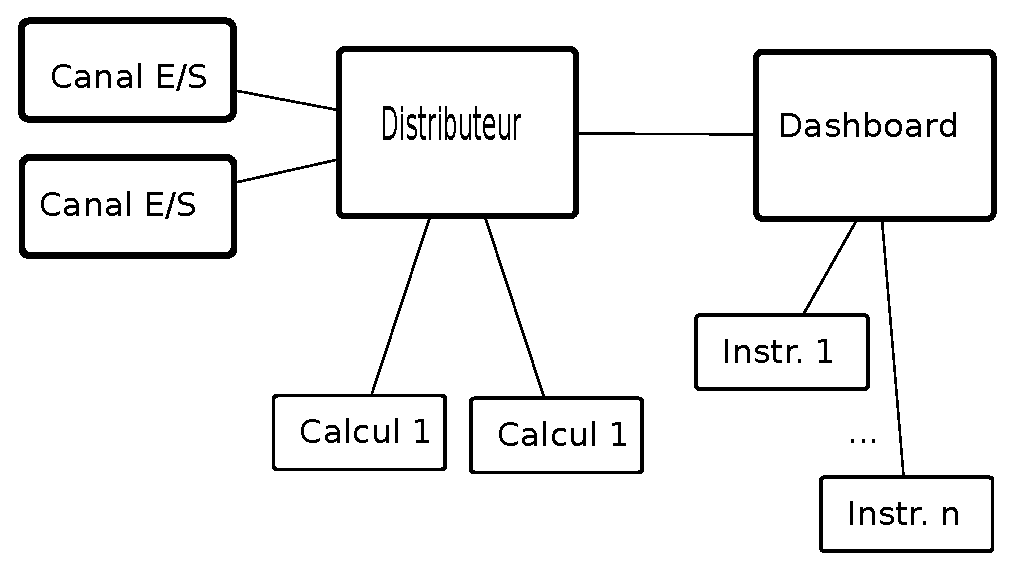
\includegraphics[width=10cm]{Conception-classes-1.eps}

La classe distributeur contient des canaux d'E/S, un tableau de bord des sorties d'export
et des modules de calculs. Le distributeur contient aussi des liens vers les instruments. 

\section {Relations dynamiques}

Les échanges entre modules se font par des messages placés dans des queues (FIFO)
ou par des fonctions membres.
 

\section{Justification des choix d'architecture}

La présence de plusieurs entrées et sorties impose l'usage de threads.
L'usage de select serait moins souple pour des versions ultérieures avec
gestion dynamique des entrées et sorties.  
tkinter impose de s'exécuter dans son propre thread.
Les calculs ont chacun leur thread pour éviter de ralentir ou bloquer
l'application en cas de calcul trop long ou infini.
\\

Cette conception modulaire facilite la maintenance et les évolutions
et surtout l'ajout de nouveaux calculs ou instruments par dérivation.

\chapter{Architecture des composants}


\section{Dashboard}

Le tableau de bord contient des instruments et une barre de contrôle en bas.



\section{Entrées sorties}

\subsection{Descripteur de fichier}
\subsection{Thread entrée}
\subsection{Thread sortie}

Le entrées et sorties sont de fichiers au sens Unix.
Ces fichiers peuvent être des périphériques (par ex. /dev/ttyUSB0), des tubes només,
voire des fichiers sur disque.
DataStream
\begin{itemize}
	\item Nom;
	\item Référence vers la queue du distributeur;
	\item Fichier.
\end{itemize}



\chapter{Description des interfaces}

\end{document}
